\subsection{Dificultades y Contratiempos}

Durante el proceso de diseño de la placa de circuito impreso se presentaron múltiples inconvenientes inesperados que tuvieron que ser resueltos para poder concretar un diseño de circuito impreso funcional. Muchos de estos inconvenientes estuvieron dados por falta de experiencia en el ámbito de diseño de PCB y utilización de software EDA, como también por problemas de disponibilidad de algunos de los componentes seleccionados a la hora del diseño circuital de la plataforma.\\

\subsubsection{Cambio de Componentes}

Muchos de los componentes a utilizar en la plataforma se eligieron durante la fase de diseño de circuitos, previo a la fase de diseño de PCB. Esto generó el dilema de que algunos componentes que se eligieron en ese momento (como el driver UCC21540 de Texas Intruments), a la hora de comenzar la PCB ya no se encontraban más en disponibilidad. Como muchos de estos componentes tenían también una disponibilidad baja y se podían acabar en cualquier momento, se decidió por elegir algunos componentes importantes y comprarlos lo antes posible, para no necesitar cambiar algunos circuitos nuevamente.\\

\subsubsection{Placa Adaptadora}

Otro inconveniente que se descubrió fue un error en el diseño de algunas de las footprints de ciertos componentes de la placa. Particularmente, en las footprints de los cuatro transistores MOSFET del puente se asignaron los pads 1, 2 y 3 a los terminales Drain (D), Gate (G) y Source (S) respectivamente, es decir que el pad central corresponde a la compuerta del transistor. Sin embargo, todos los transistores MOSFET de potencia compatibles con esta footprint tienen una configuración de pines del tipo Gate - Drain - Source, con los pines Gate y Drain (1 y 2) invertidos respecto a la footprint presente en la PCB.\\

La solución obvia sería simplemente modificar el archivo de la placa para corregir este error. Sin embargo, el problema se encuentra en que el error se descubrió una vez enviados los archivos Gerber al fabricante de circuitos impresos y ya comenzado el proceso de fabricación, por lo que se debió idear alguna otra solución al dilema.\\

\begin{figure}[h]
    \centering
    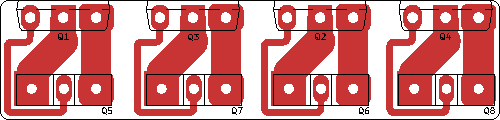
\includegraphics[scale=1.3]{Imagenes/Placa Adaptadora.pdf}
    \caption{Capa de cobre de la placa adaptadora diseñada para mitigar el error de diseño.}
    \label{fig:placa_adaptadora}
\end{figure}

La solución implementada se aprecia en la figura \ref{fig:placa_adaptadora}: una placa adaptadora con una única capa de cobre, que se conecta a los pads de los transistores en la placa original, y mediante las pistas de cobre visibles en la figura se conecta a una nueva footprint, con los pads en el orden correcto. La placa se diseño de manera que no estorbe con componentes cercanos a los transistores (como el conector de la pila de combustible), y lo suficientemente pequeña para no sobresalir significativamente de la placa original y permitir la instalación del disipador metálico. También se eligió de simple capa para facilitar su fabricación, pudiéndose entonces fabricar en la sala del ATEI dentro de la Facultad de Ingeniería, proceso que es de mucho menor costo y tiempo de fabricación.\\

